\documentclass[12pt]{article}
\usepackage[left=1in, right=1in, top=1in, bottom=1in]{geometry}
\usepackage{titling}

\usepackage{graphicx}
\usepackage[export]{adjustbox}
\usepackage{caption}
\usepackage{subcaption}
\usepackage{hyperref}

\renewcommand{\arraystretch}{1.5}

\hypersetup{
    colorlinks=true,
    linkcolor=blue,
    filecolor=magenta,      
    urlcolor=cyan,
}

\graphicspath{ {images/} }

\setlength{\droptitle}{-5em} 
\pretitle{\begin{center}\Huge\bfseries}
\posttitle{\par\end{center}\vskip 0.5em}
\preauthor{\begin{center}\Large\ttfamily}
\postauthor{\end{center}}
\predate{}
\postdate{}

\title{Demucs \\ \large Neural Networks project}
\author{Simone Bartolini 1752197}
\date{}
\begin{document}

\maketitle
\thispagestyle{empty}



\section{Introduction}\label{sec:intro}
For this project, I've reimplemented in a simplified form the first version of the Demucs neural network, a model for music source separation. It has been proposed in the paper \cite{Defossez_2019} and the source code is available on GitHub \cite{Demucs_code}.\\
I've coded my version using python and the PyTorch library and trained it using Google Colab to have access to more powerful hardware than the one I have in my computer. My source code is also available on \href{https://github.com/51m0n397/NN-project/tree/main/code}{GitHub}. \\
In the rest of this document: 
\begin{itemize}
\item I describe the structure of the network and the changes I made with respect to the model presented in the paper in \autoref{sec:model};
\item I detail the dataset generation and data augmentation in  \autoref{sec:data};
\item I define the training procedure in \autoref{sec:train};
\item I discuss the evaluation technique and compare my results to the one in the paper in \autoref{sec:res};
\item I provide my closing thoughts in \autoref{sec:conclusion}.
\end{itemize}


\newpage
\section{Model}\label{sec:model}
Demucs is an 
\begin{quote}
\textit{encoder/decoder architecture composed of a convolutional encoder, a bidirectional LSTM, and a convolutional decoder, with the encoder and decoder linked with skip U-Net connections \cite{Defossez_2019}.}
\end{quote}
It takes in input a stereo mixture and produces in output four stereo tracks, one for each source (\textit{vocals}, \textit{drums}, \textit{bass} and \textit{others}).\\\\
The network is structured as follows (figure \ref{fig:model}):
\begin{itemize}
\item The encoder is made of six blocks, numbered from 1 to 6, each composed of a convolution with a kernel size of 8, a stride of 4 and ReLU activation and another convolution with a kernel size of 1, a stride of 1 and GLU activation. The first convolution produces in output \(2^{i-1}*C\) channels, where \(i\) is the block number and \(C=64\), while the second convolution at first doubles the output channels but then the GLU activation layer halves it again, thus the final output of the block is still \(2^i*C\) channels. The first block takes in input the two channels of the input mixture, while the remaining blocks take in input the output channels of the preceding block.
\item The bidirectional LSTM has two layers and a hidden size equal to the number of output channels of the encoder, i.e., 2048. The 4096 output channels of the LSTM are then passed through a linear layer that halves them to 2048.
\item The decoder is also made of six blocks, this time numbered from 6 to 1, each one composed of a convolution with a kernel size of 3, a stride of 1 and GLU activation and a transposed convolution with a kernel size of 8, a stride of 4 and ReLU activation. The first block takes in input the 2048 channels outputted by the linear layer, while the remaining blocks take in input the output channels of the preceding block. Additionally, the input of each decoder block is summed with the output of the relative encoder block with the same number (skip U-Net connections). Inside each block, the first convolution produces in output \(2^{i}*C\) channels, where \(i\) is the block number and \(C=64\), that get halved by the GLU activation and then halved again by the second convolution, thus the whole block produces in output \(2^{i-2}*C\) channels, except for the last block, where the transposed convolution gives in output 8 channels, i.e., two channels for each of the four output tracks.
\end{itemize}
Note that the original model had C=100, but to reduce the size of the model I've changed it to 64, as suggested in the source to make it possible to train the model on a system with a limited amount of RAM and VRAM.


\begin{figure}[h!]
\centering

\begin{subfigure}{1\textwidth}
  \captionsetup{justification=centering}
  \centering
  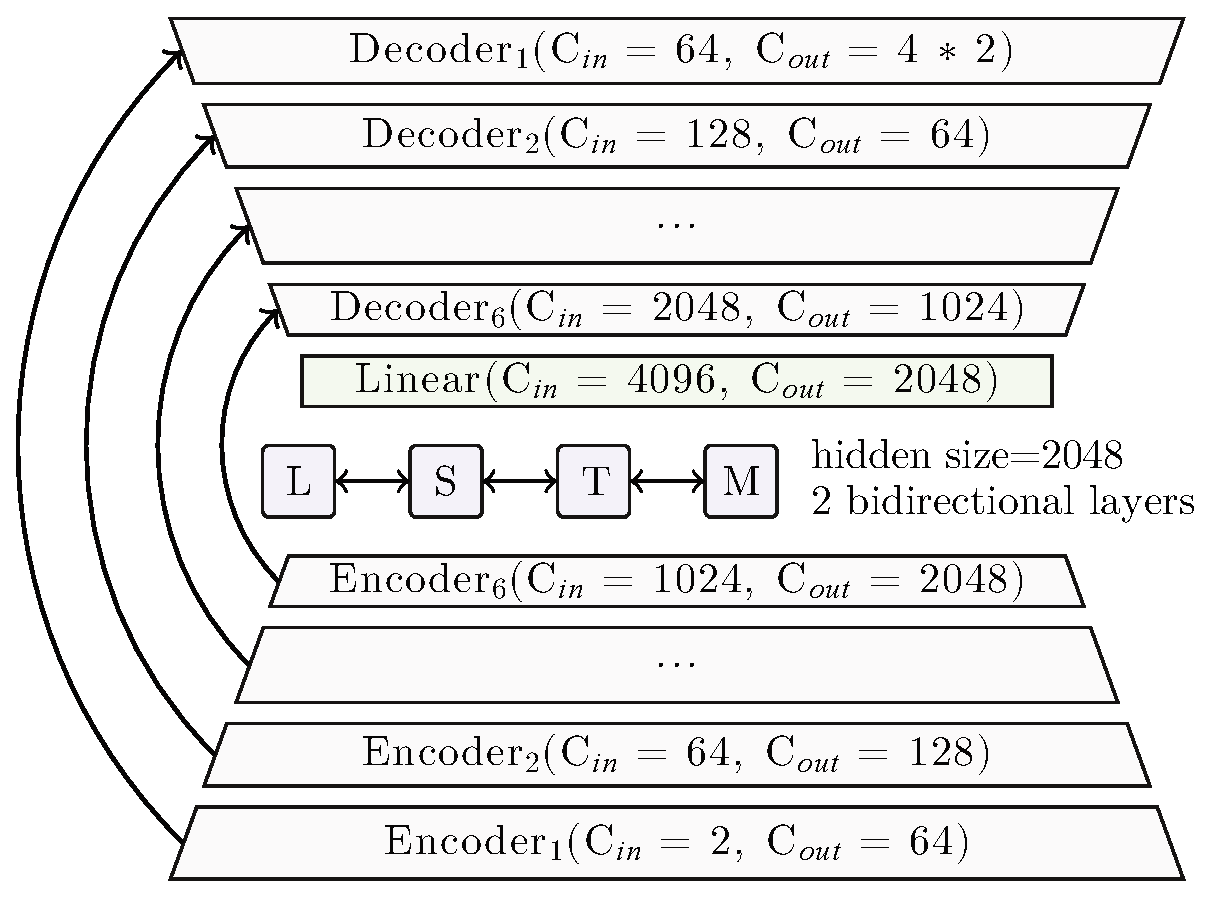
\includegraphics[width=.7\linewidth]{modelA}
  \caption{Demucs architecture (modified version of the image in \cite{Defossez_2019}).}
  \label{fig:modelA}
\end{subfigure}%

~\\~\\~

\begin{subfigure}{1\textwidth}
  \captionsetup{justification=centering}
  \centering
  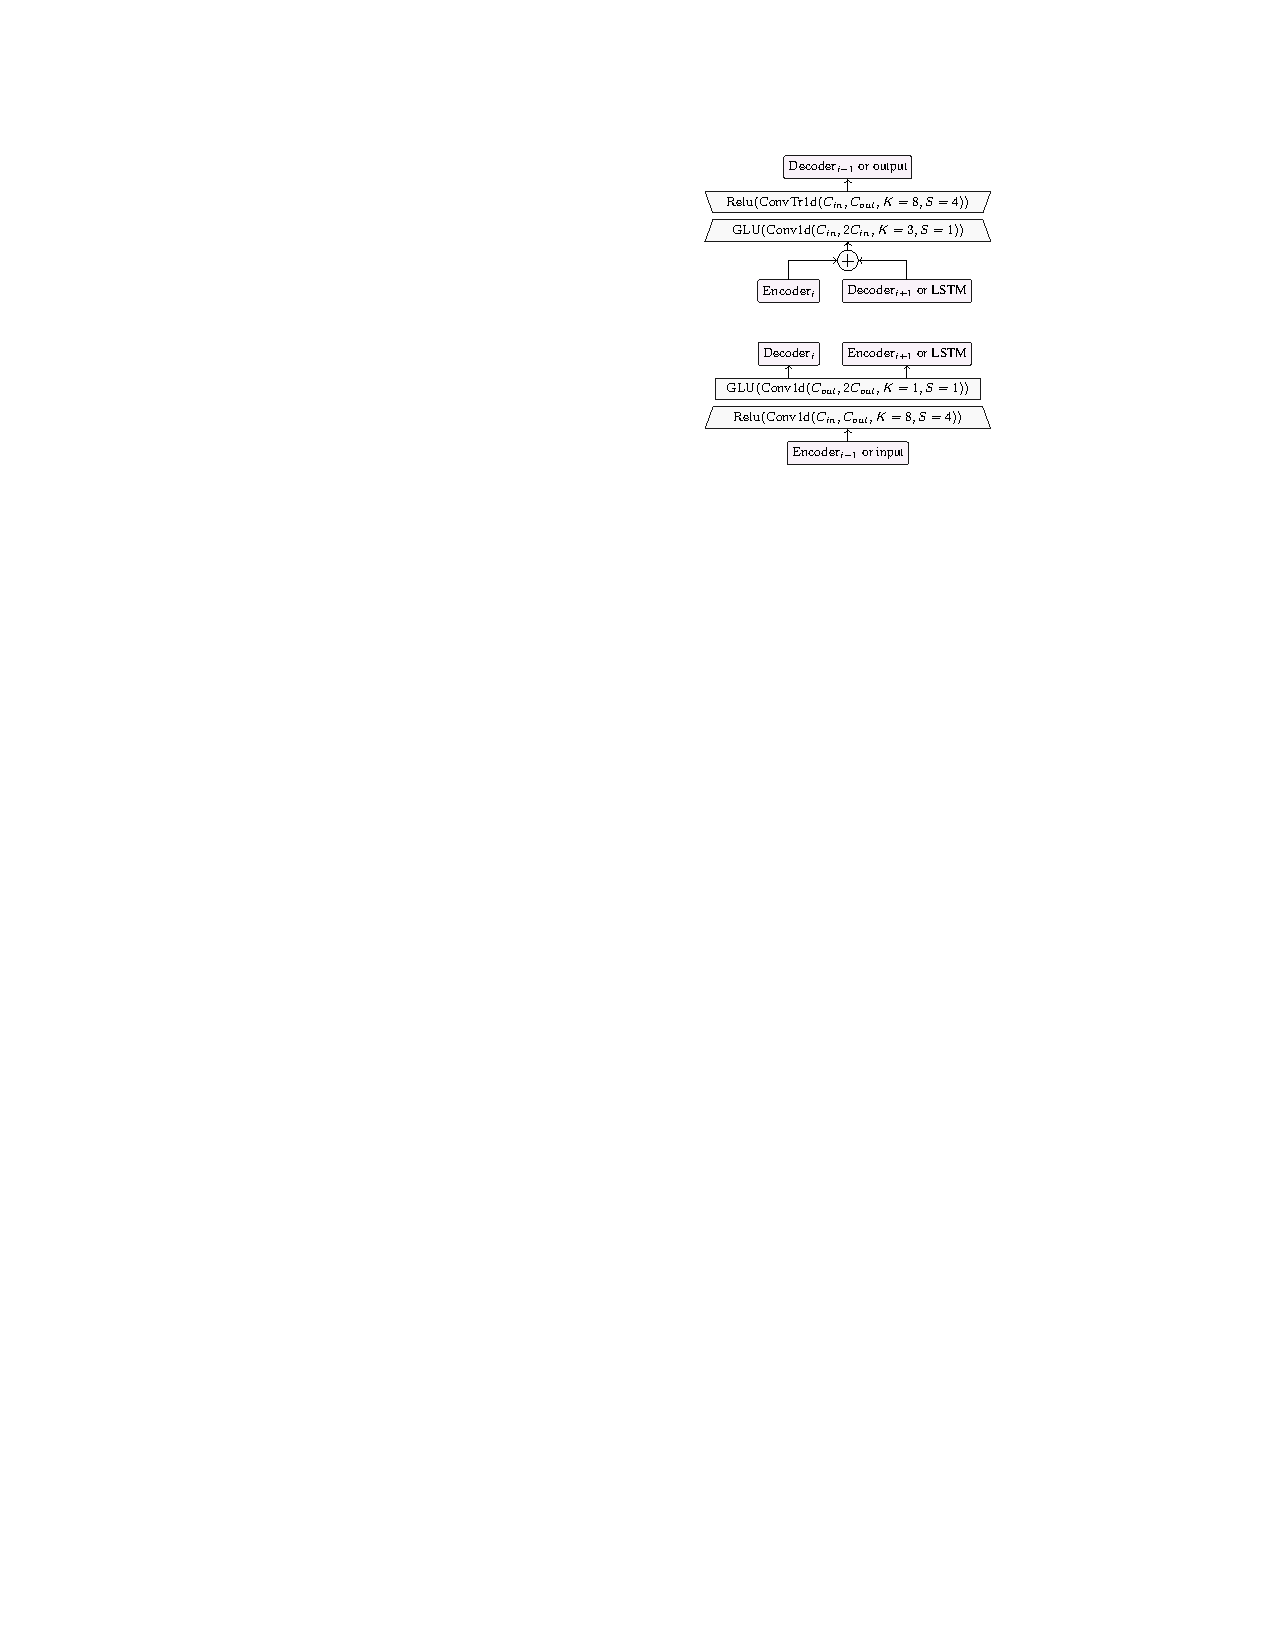
\includegraphics[width=.5\linewidth]{modelB}
  \caption{Detailed view of a decoder (top) and an encoder (bottom) block \cite{Defossez_2019}.}
  \label{fig:modelB}
\end{subfigure}

\caption{Model}
\label{fig:model}
\end{figure}

\newpage
\section{Dataset}\label{sec:data}
The model has been trained on the \textit{musdb18} dataset \cite{musdb18}. \textit{musdb18} is a dataset of 150 stereo songs, purposely developed for training and evaluation of source separation models. For each song it contains the full mixture plus the separate tracks for the sources (\textit{vocals}, \textit{drums}, \textit{bass} and \textit{others}), that summed together form the mixture. The dataset is divided into 84 songs for training, 16 songs for validation and 50 songs for testing.\\
In the original code, the songs were passed in input to the network as 11-second extracts with a stride of 1 second. This resulted in extremely long training time (multiple days) on the hardware I've access to, i.e. an Nvidia Tesla K4 with 16GB of VRAM obtained through Google Colab (note that the original network has been trained on 16 Nvidia V100 GPUs, each with 32GB of VRAM). For this reason, I've decided to extract at random only a limited number of 11-seconds chunks from each song, specifically 1.25 chunks per minute of song, effectively reducing the size of the dataset and thus the training time to around 6 hours (of course at the cost of the performance of the trained model).\\
The data is normalized using z-score normalization, i.e., the mean of each song is subtracted from every 11-second chunk extracted from it, and the result is divided by the standard deviation of the song. After that, each chunk is shifted in time by a random number between 0 and 1 and only 10 seconds are kept.\\
Then the following data augmentation is performed:
\begin{itemize}
\item randomly flipping the audio channels;
\item randomly flipping the sign;
\item shuffling the sources within a batch.
\end{itemize}

 

\newpage
\section{Training}\label{sec:train}
\subsection{Weight initialization}
Correctly initializing the weight of the network can have a huge impact on performance. The authors of the paper take a peculiar approach: the weight of the convolutions are initialized at random and then rescaled in order to get their standard deviation closer to a target value of \(a=0.1\). This is done as follows: let's denote with \(w\) the initial value of a weight. We then compute \(\alpha=\mathrm{std}(w)/a\) and replace \(w\) with \(w'=w/\sqrt\alpha\).

\subsection{Loss function}
The paper suggests two possible loss functions to use:
\begin{enumerate}
\item the average absolute error \(L_{1}\left(\hat{x}_{s}, x_{s}\right)=\frac{1}{T} \sum_{t=1}^{T}\left|\hat{x}_{s, t}-x_{s, t}\right|\);
\item the average mean square error \(L_{2}\left(\hat{x}_{s}, x_{s}\right)=\frac{1}{T} \sum_{t=1}^{T}\left(\hat{x}_{s, t}-x_{s, t}\right)^{2}\);
\end{enumerate}
where \(x_{s}\) is a waveform containing \(T\) samples corresponding to the source \(s\), \(\hat{x}_{s}\) is a predicted waveform and the subscript \(t\) denotes the \(t\)-th sample of a waveform.\\
I've trained and evaluated the model using both loss functions.

\subsection{Training cycle}
After the initialization, the model is trained using the Adam trainer for 240 epochs with a learning rate of \(3e-4\) and passing the data examples in input at batches of 8 (note that this is reduced from the original batch size of 64, again due to memory limitation of the hardware at my disposal).\\
The images below (figures \ref{fig:training1} and \ref{fig:training2}) describe the evolution of the loss over the course of the training for the two variants (note that I've computed the validation loss only every 10 epochs).


\newpage

\begin{figure}[h]
  \centering
  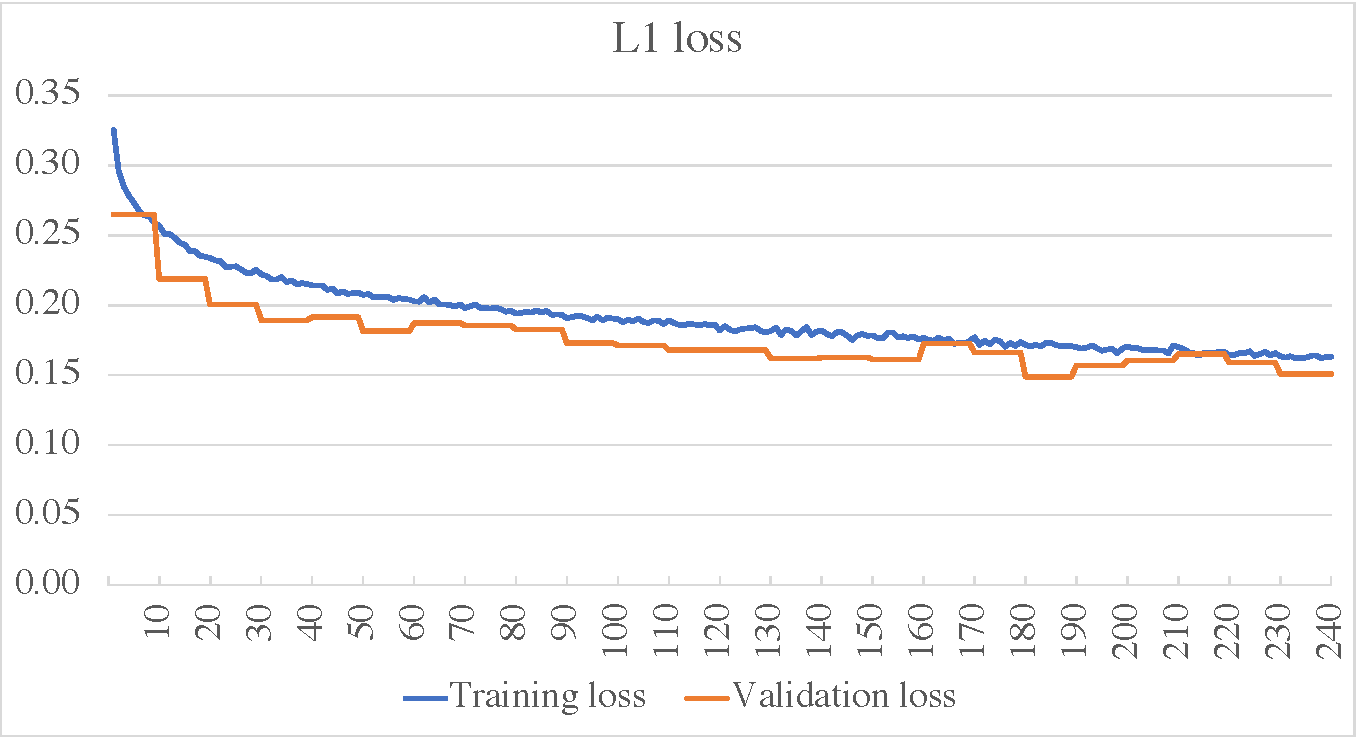
\includegraphics[width=1\linewidth]{l1}
  \caption{L1 loss during training}
  \label{fig:training1}
\end{figure}

~

\begin{figure}[h!]
  \centering
  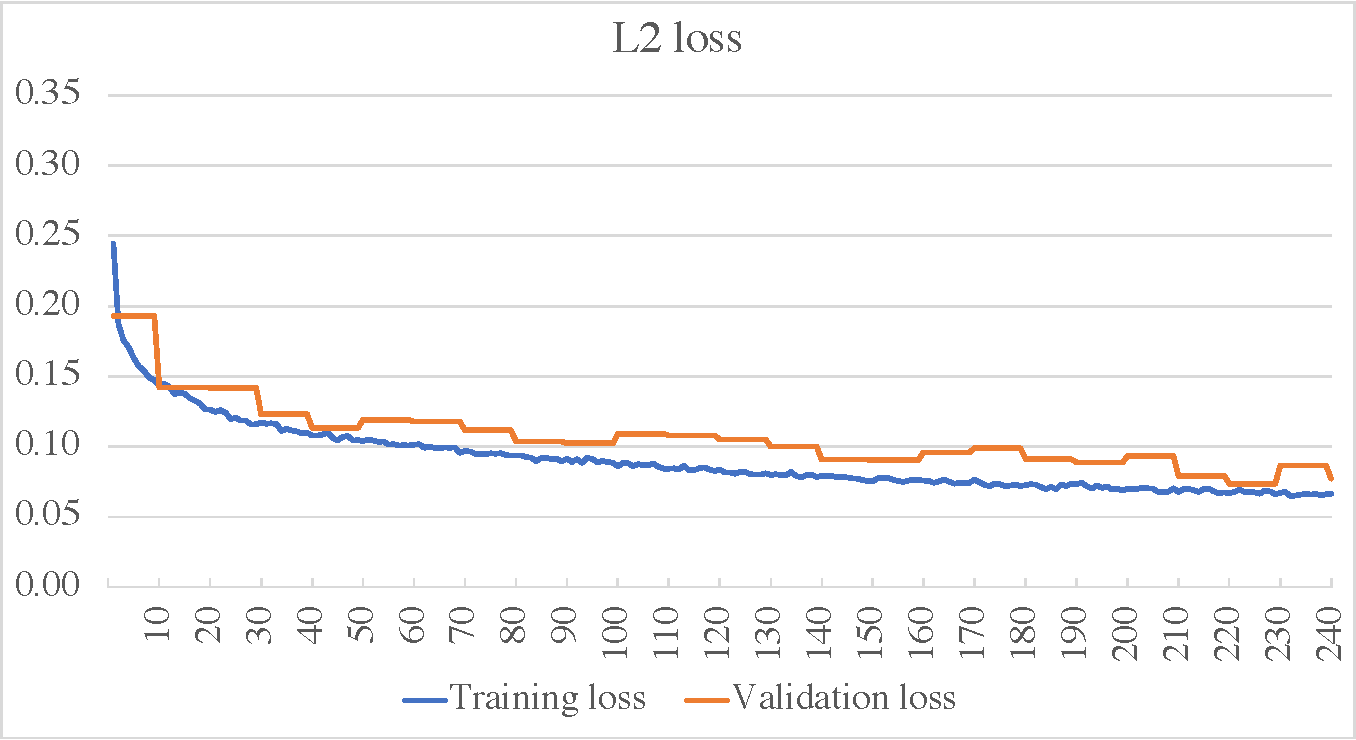
\includegraphics[width=1\linewidth]{l2}
  \caption{L2 loss during training}
  \label{fig:training2}
\end{figure}



\newpage
\section{Results}\label{sec:res}
\subsection{The shift trick}
As is, the Demucs model is not time equivariant, i.e., shifting the input mixture by X samples will not shift the output by the same amount. This reduces the accuracy of the model. To mitigate the problem, the paper suggests a simple workaround called \textit{randomized equivariant stabilization} (or also the \textit{shift trick}) that consist of sampling \(S=10\) random shifts of an input mixture and averaging the prediction of the model for each, after having applied the opposite shift, to compute the final output. Note that this is only done during evaluation and not training as it would substantially increase the time required.

\subsection{Evaluation procedure}
The evaluation is done using the 50 testing songs in the dataset. First, the average loss (either L1 or L2, depending on which has been used for training) is computed, then the predictions are analyzed using the \texttt{museval} python package \cite{fabian_robert_stoter_2021_4486535}, which implements the SiSec Mus 2018 \cite{SiSEC18} evaluation that is used in literature for evaluating source separation models trained over the \textit{musdb18} dataset. The package computes four metrics for each source:
\begin{itemize}
\item Source to Distortion ratio (SDR);
\item Source to Artefact ratio (SAR);
\item Source to Interference ratio (SIR);
\item Image to Spatial distortion ratio (ISR).
\end{itemize}
These metrics are computed for each sample of each song and the final result is the median over all songs. Out of the four metrics, the primary one used to judge the quality of the source separation is the SDR. The tables below (tables \ref{tab:results1} and \ref{tab:results2}) show the results for each of the four output tracks plus the average over all tracks.


\begin{table}[h]
\centering
\begin{tabular}{l|l|llll}
                 & \textbf{All}            & \multicolumn{1}{l|}{\textbf{Vocals}} & \multicolumn{1}{l|}{\textbf{Drums}} & \multicolumn{1}{l|}{\textbf{Bass}} & \textbf{Other} \\ \hline
\textbf{SDR}     & \textit{\textbf{3.961}} & \multicolumn{1}{l|}{3.137}           & \multicolumn{1}{l|}{5.302}          & \multicolumn{1}{l|}{5.291}         & 2.113          \\ \hline
\textbf{SAR}     & 4.872                   & \multicolumn{1}{l|}{3.387}           & \multicolumn{1}{l|}{6.105}          & \multicolumn{1}{l|}{5.418}         & 4.577          \\ \hline
\textbf{SIR}     & 7.274                   & \multicolumn{1}{l|}{8.636}           & \multicolumn{1}{l|}{8.783}          & \multicolumn{1}{l|}{9.229}         & 2.446          \\ \hline
\textbf{ISR}     & 7.427                   & \multicolumn{1}{l|}{5.086}           & \multicolumn{1}{l|}{8.611}          & \multicolumn{1}{l|}{9.211}         & 6.798          \\ \hline
\textbf{L1 loss} & 0.194                   &                                      &                                     &                                    &               
\end{tabular}
\caption{Results of training using L1 loss}
\label{tab:results1}
\end{table}


\begin{table}[h]
\centering
\begin{tabular}{l|l|llll}
                 & \textbf{All}            & \multicolumn{1}{l|}{\textbf{Vocals}} & \multicolumn{1}{l|}{\textbf{Drums}} & \multicolumn{1}{l|}{\textbf{Bass}} & \textbf{Other} \\ \hline
\textbf{SDR}     & \textit{\textbf{3.928}} & \multicolumn{1}{l|}{3.663}           & \multicolumn{1}{l|}{5.077}          & \multicolumn{1}{l|}{4.479}         & 2.494          \\ \hline
\textbf{SAR}     & 5.534                   & \multicolumn{1}{l|}{4.876}           & \multicolumn{1}{l|}{5.300}          & \multicolumn{1}{l|}{6.896}         & 5.064          \\ \hline
\textbf{SIR}     & 5.936                   & \multicolumn{1}{l|}{7.438}           & \multicolumn{1}{l|}{6.177}          & \multicolumn{1}{l|}{7.467}         & 2.662          \\ \hline
\textbf{ISR}     & 7.722                   & \multicolumn{1}{l|}{6.375}           & \multicolumn{1}{l|}{9.519}          & \multicolumn{1}{l|}{8.705}         & 6.287          \\ \hline
\textbf{L2 loss} & 0.103                   &                                      &                                     &                                    &               
\end{tabular}
\caption{Results of training using L2 loss}
\label{tab:results2}
\end{table}




\subsection{Results analysis}
As the results highlight, the model trained using the L1 loss performs slightly better on average, although the L2 variant separated better the \textit{vocals} and \textit{other} tracks. Also the authors of the paper found a small improvement when using the L1 loss, with an average SDR of 5.58 compared to 5.55 when using L2. \\
The table \ref{tab:results-original} shows the SDR, SAR, SIR and L1 loss of the original model (note that the ISR is missing because it was not reported in the paper). The changes I made to make it possible to train the model on less powerful hardware definitely had an impact on the quality of the separation, especially with the \textit{vocals} and \textit{other} tracks, which is not surprising as they are the most difficult to separate. This is consistent with what I can hear listening to some of the output tracks of my model compared to the original: while the \textit{drums} and \textit{bass} tracks are mostly ok, there is a lot of cross bleeding in the \textit{vocals} and \textit{other} tracks, definitely more than in the output of the original model (although even that struggles a bit with separating the two).

\begin{table}[h]
\centering
\begin{tabular}{l|l|llll}
                 & \textbf{All}           & \multicolumn{1}{l|}{\textbf{Vocals}} & \multicolumn{1}{l|}{\textbf{Drums}} & \multicolumn{1}{l|}{\textbf{Bass}} & \textbf{Other} \\ \hline
\textbf{SDR}     & \textit{\textbf{5.58}} & \multicolumn{1}{l|}{6.29}            & \multicolumn{1}{l|}{6.08}           & \multicolumn{1}{l|}{5.83}          & 4.12           \\ \hline
\textbf{SAR}     & 6.08                   & \multicolumn{1}{l|}{6.54}            & \multicolumn{1}{l|}{6.18}           & \multicolumn{1}{l|}{6.41}          & 5.18           \\ \hline
\textbf{SIR}     & 10.39                  & \multicolumn{1}{l|}{13.31}           & \multicolumn{1}{l|}{11.81}          & \multicolumn{1}{l|}{10.55}         & 5.90           \\ \hline
\textbf{L1 loss} & 0.164                  &                                      &                                     &                                    &               
\end{tabular}
\caption{Results of training of the original model}
\label{tab:results-original}
\end{table}

\newpage
\section{Conclusion}\label{sec:conclusion}
Demucs can achieve really impressive results in the separation of music sources. My reimplementation falls shorts of reaching the same quality due to the aforementioned reduction of the size of the model and of the dataset, although it requires significantly less powerful hardware and time to train. With more time at my disposal, it could be interesting to test if it is possible to achieve better results with my model by changing parameters like the learning rate or the rescale factor \(a\) at initialization, or by increasing the training epochs since the validation loss did not show signs of overfitting.

\newpage
\bibliographystyle{sapthesis}
\bibliography{bib} 

\end{document}